% =====================================================================
%  AI251P Applied Computer Vision -- Capstone Project
%  Phase 2 Report Template (M4, M5, M8, 45 points, due 15 November 2026)
%
%  How to use:
%   * Fill in the team details in the "TEAM DETAILS" block below.
%   * Replace every grey italic prompt (\prompt{...}) with your own text.
%   * Adapt the methods to your problem: the prompts say what must be
%     shown, and the "e.g." hints are examples, not required steps.
%   * Fill every table. Add, remove or rename rows and columns to fit
%     your task, and say why when something does not apply.
%   * Put your figures in the figures/ folder and replace
%     figures/placeholder.png with your own file names.
%   * Every reported figure must state the data split, the input
%     resolution and the thresholds used.
%   * "Optional extras" are not required for full credit.
%   * Teams of 5 must also complete Section 5 (Open-world extension).
%     Teams of 3 or 4 delete Section 5.
% =====================================================================
\documentclass[11pt,a4paper]{article}

\usepackage[T1]{fontenc}
\usepackage[utf8]{inputenc}
\usepackage{mathpazo}
\usepackage[margin=2.2cm]{geometry}
\usepackage{booktabs,tabularx,array,multirow}
\usepackage{graphicx}
\usepackage{caption}
\usepackage{float}
\usepackage{enumitem}
\usepackage{amsmath,amssymb}
\usepackage{xcolor}
\usepackage{fancyhdr}
\usepackage[colorlinks=true,linkcolor=blue!50!black,urlcolor=blue!50!black]{hyperref}

% ---------------------------------------------------------------------
%  TEAM DETAILS -- edit these
% ---------------------------------------------------------------------
\newcommand{\teamname}{Smart Pet Vision}
\newcommand{\projecttitle}{Smart Pet Vision: Pet Photo Review Assistant for Shelters}

% ---------------------------------------------------------------------
%  Helpers
% ---------------------------------------------------------------------
% Grey italic prompt: delete it and write your own text in its place.
\newcommand{\prompt}[1]{\leavevmode{\color{gray!80!black}\itshape #1}}
% Blank line for short answers
\newcommand{\blank}{\rule{0pt}{2.2ex}}
% Points label in section titles: \pts{teams of 3-4}{teams of 5}
\newcommand{\pts}[2]{\texorpdfstring{\hfill{\normalsize\mdseries(#1 points; teams of 5: #2)}}{}}
\newcommand{\ptsone}[1]{\texorpdfstring{\hfill{\normalsize\mdseries(#1 points)}}{}}
% Heading for optional material
\newcommand{\optextras}{\subsection*{Optional extras {\normalsize\mdseries\itshape(not required for full credit)}}}
% Threshold symbols
\newcommand{\tconf}{$\tau_{\text{conf}}$}
\newcommand{\tnms}{$\tau_{\text{NMS}}$}
% Checklist
\newlist{checklist}{itemize}{1}
\setlist[checklist]{label=$\square$,leftmargin=1.6em,itemsep=2pt}
\newcolumntype{Y}{>{\raggedright\arraybackslash}X}
\renewcommand{\arraystretch}{1.25}
\setlength{\parindent}{0pt}
\setlength{\parskip}{4pt}

\pagestyle{fancy}
\fancyhf{}
\lhead{\itshape AI251P Applied Computer Vision}
\rhead{\itshape Capstone Phase 2 Report -- \teamname}
\cfoot{\thepage}
\setlength{\headheight}{14pt}

\newcommand{\run}[1]{\href{https://wandb.ai/yasser-alhajlah-kaust/smart-pet-vision/runs/#1}{\texttt{#1}}}
\newcommand{\code}[1]{\texttt{\detokenize{#1}}}

% Student IDs are kept out of the public repository (instructor rule: no personal
% information in the repo). Put private_ids.tex next to this file to fill them in.
\IfFileExists{private_ids.tex}{\input{private_ids.tex}}{%
  \newcommand{\idYasser}{(ID)}\newcommand{\idMohammed}{(ID)}%
  \newcommand{\idMusaad}{(ID)}\newcommand{\idAbdulrahman}{(ID)}}

\begin{document}

% =====================================================================
\begin{center}
  {\large AI251P Applied Computer Vision}\\[4pt]
  {\LARGE\bfseries Capstone Project -- Phase 2 Report}\\[6pt]
  {\Large \projecttitle}\\[4pt]
  \teamname\ \textperiodcentered\ Phase 2 (M4, M5, M8, 45 points) \textperiodcentered\ Due 15 November 2026
\end{center}
\vspace{4pt}

% =====================================================================
\section{Team and system}

\begin{tabularx}{\linewidth}{@{}l Y@{}}
\toprule
Field & Our answer \\
\midrule
Team name & Smart Pet Vision \\
Team size & 4 (Section 5, open-world extension, is therefore omitted) \\
Topic & Original topic, approved by the instructor (19 October 2026): pet photo review for shelter adoption listings \\
Code repository and commit hash & \url{https://github.com/Yasser-20-alhajlah/smart-pet-vision} \;\; \texttt{d395488} (Phase 2 code in \texttt{smart-pet-vision/phase2/}) \\
W\&B project & \url{https://wandb.ai/yasser-alhajlah-kaust/smart-pet-vision} \\
Deployed service / demo & Run locally or in Colab: \texttt{SPV\_MANIFEST=runs/manifest.json uvicorn spv.serve:app --port 8000} from \texttt{smart-pet-vision/phase2/src}; full steps in \texttt{phase2/README.md} and notebook \texttt{06\_release\_validation\_v2.ipynb} \\
Model card & \href{https://github.com/Yasser-20-alhajlah/smart-pet-vision/blob/main/smart-pet-vision/phase2/docs/model_card.md}{\texttt{phase2/docs/model\_card.md}} in the repository \\
\bottomrule
\end{tabularx}

\subsection*{Team members}

\begin{tabularx}{\linewidth}{@{}l l l Y@{}}
\toprule
Name & Student ID & Workstream & Phase 2 contribution \\
\midrule
Yasser Mansour Alhajlah & \idYasser{} & 2. Detection & Body-box conversion and checks, YOLO11s fine-tuning, threshold sweep, error analysis, video inference \\
Mohammed Adeeb Alrashdi & \idMohammed{} & 3. Segmentation & Trimap mask targets, SAM 2.1 reference, YOLO11s-seg fine-tuning and evaluation \\
Musaad Obaied Saad Alqahtani & \idMusaad{} & 4. Integration & Pipeline and manifest, FastAPI service, ONNX export and parity, benchmarks \\
Abdulrahman Mastour Alharthi & \idAbdulrahman{} & 1. Data and classification & Phase 1 classifier in the verdict rule, label integrity, team-photo evaluation set \\
\bottomrule
\end{tabularx}

\subsection*{Points by team size}

\begin{tabularx}{\linewidth}{@{}Y c c@{}}
\toprule
Component & Teams of 3--4 & Teams of 5 \\
\midrule
Object detection (M4) & 15 & 12 \\
Segmentation (M5) & 15 & 12 \\
Integration and deployment (M8) & 15 & 11 \\
Open-world extension (two topics, 5 points each) & -- & 10 \\
\midrule
\textbf{Total} & \textbf{45} & \textbf{45} \\
\bottomrule
\end{tabularx}

\subsection*{System overview}

\begin{figure}[H]
  \centering
  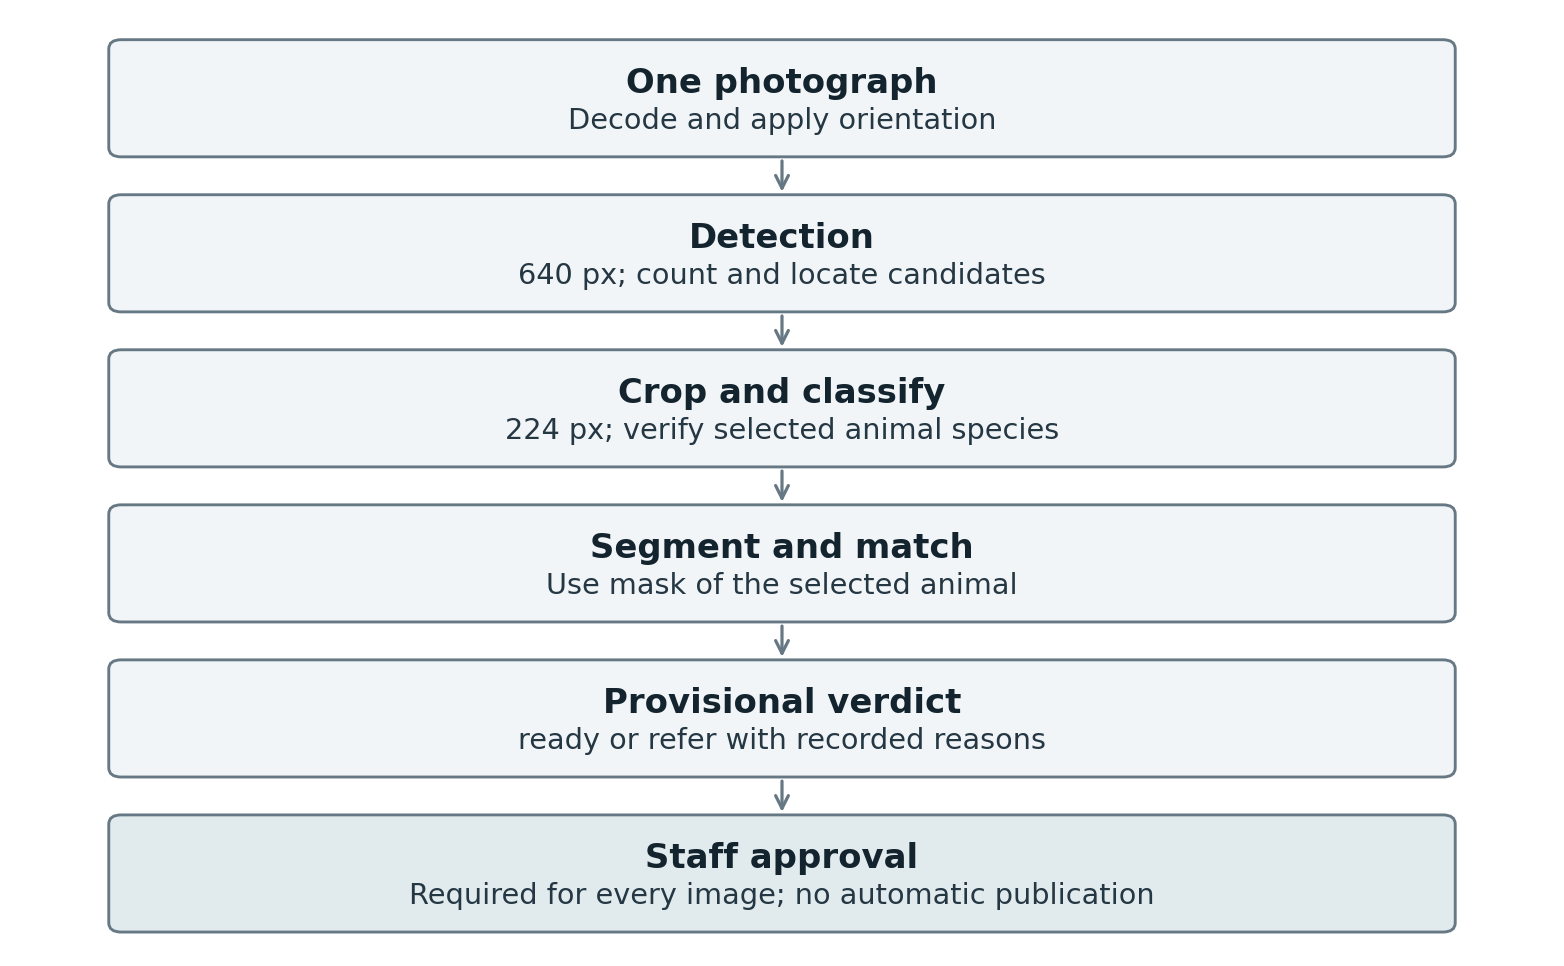
\includegraphics[width=0.82\linewidth]{figures/pipeline_flow.png}
  \caption{End-to-end pipeline for one uploaded photo: detection (640\,px, \tconf{} 0.40, \tnms{} 0.50), classification of the selected crop (224\,px, temperature 0.05, verification threshold 0.90), segmentation (640\,px) and the referral rule. Every verdict, ready or referred, goes to a staff member for approval.}
\end{figure}

{\small
\begin{tabularx}{\linewidth}{@{}l l Y Y Y@{}}
\toprule
Component & Model & Input & Output & Function in the system \\
\midrule
Classifier (Phase 1) & ResNet-50, fine-tuned & 224\,px crop of the selected box & Cat/dog probabilities (temperature-scaled) & Confirms the detector's species; disagreement or confidence $<0.90$ triggers referral \\
Detector (M4) & YOLO11s, fine-tuned & Photo, letterboxed to 640\,px & Body boxes with species and score & Counts animals (0 or $\geq2$ $\rightarrow$ referral) and selects the crop \\
Segmentation (M5) & YOLO11s-seg, fine-tuned & Photo, letterboxed to 640\,px & Instance masks & Matches a mask to the selected animal; mask share $<0.05$, no match or a second animal $\rightarrow$ referral \\
\bottomrule
\end{tabularx}}

\subsection*{Acceptance criteria (fixed in Phase 1)}

A1--A2 are the criteria of the Phase 1 report. A3--A8 and A9a were written in the team's integration notebook (code snapshot of 15 October 2026, before the first Phase 2 run on 17 October); A9b, the same bound applied to the detector, was added no later than the first integration run. None was changed after results were seen. The values are computed by notebook \texttt{05\_integration.ipynb} into \texttt{evidence/M8\_acceptance.csv}, and \texttt{tools/verify\_submission\_evidence.py} checks that the numbers in this report match the saved evidence.

{\small
\begin{tabularx}{\linewidth}{@{}l Y l l Y@{}}
\toprule
ID & Criterion & Metric & Threshold & Conditions (split, hardware, settings) \\
\midrule
A1 & Species classification & Accuracy & $\geq 0.90$ & Oxford test, 224\,px, argmax (Phase 1) \\
A2 & Species classification & Macro-F1 & $\geq 0.90$ & As A1 (Phase 1) \\
A3 (added) & Body detection & mAP50 & $\geq 0.75$ & Oxford test, 640\,px, evaluation \tconf{} 0.001 \\
A4 (added) & Body detection & Recall & $\geq 0.80$ & Oxford test, operating point \tconf{} 0.40, \tnms{} 0.50 \\
A5 (added) & Body mask & Mean IoU & $\geq 0.75$ & Oxford test, 640\,px, mask \tconf{} 0.25 \\
A6 (added) & Body mask & Mean Dice & $\geq 0.85$ & As A5 \\
A7 (added) & Service & HTTP success rate & $\geq 0.99$ & 300 requests, uvicorn, PyTorch backend \\
A8 (added) & Latency & p95 end to end & $\leq 2000$\,ms & T4, batch 1, PyTorch, after 10 warm-up \\
A9a (added) & Classifier export & Max abs diff & $\leq 0.001$ & PyTorch vs ONNX, CPU \\
A9b (added) & Detector export & Max abs diff & $\leq 0.001$ & PyTorch vs ONNX raw head, CPU, 4 inputs, seed 0 \\
\bottomrule
\end{tabularx}}

\subsection*{Follow-up on the Phase 1 data-improvement plan}

{\small
\begin{tabularx}{\linewidth}{@{}Y l Y@{}}
\toprule
Planned action (Phase 1) & Done? & Measured effect \\
\midrule
Collect harder images (puppies, curled-up, clothed, multiple, small animals) & No & No new photos were collected in Phase 2. The 401 team photos stay an evaluation-only set. Their detector results (Section~\ref{sec:team}) confirm the need: recall 0.732, small-animal bin 0/10 found \\
Rebalance cats and dogs; add hairless and colour-point cats & No & Not done; the split is still about 1:2. Siamese is among the five weakest breeds for masks (IoU 0.899) \\
Fit the temperature on a harder calibration set & No & Needs the new photos above. The service keeps $T=0.05$ from Phase 1, so its confidence is not claimed as calibrated on new photos \\
Re-derive the four loose body boxes; add a box-quality check & Partly & Round-trip check on all 7,335 YOLO labels (0 missing, 0 class mismatches); the four boxes were not re-derived \\
\bottomrule
\end{tabularx}}

% =====================================================================
\section{Object detection (M4)\pts{15}{12}}

\textbf{Task:} detect the whole body of each cat and dog in the photo (two classes). The detections count the animals (none or several $\rightarrow$ referral), give the box for the classifier crop and the species that the classifier must confirm.

Models, thresholds and settings were chosen on the validation split; the test split was evaluated once.

\subsection{Annotation conversion and verification}

Oxford-IIIT Pet provides a head box and a pixel trimap. The head box does not cover the body, so the body box is the tightest box around the trimap foreground plus border.

\begin{tabularx}{\linewidth}{@{}Y l Y@{}}
\toprule
Item & Count & Notes \\
\midrule
Source format $\rightarrow$ target format & -- & Trimap PNG $\rightarrow$ body box $\rightarrow$ YOLO txt (normalised centre, width, height) \\
Boxes converted & 7,335 & One animal per Oxford image \\
Boxes fixed (e.g.\ clipped to the image) & 0 & Boxes are derived inside the image, so none needed clipping \\
Boxes or objects removed, and why & 14 images & Empty trimap, removed in Phase 1 cleaning (7,349 received) \\
Background images (no objects) & 0 & Every Oxford image contains one animal \\
\bottomrule
\end{tabularx}

\medskip
\begin{tabularx}{\linewidth}{@{}l r r Y@{}}
\toprule
Split & Images & Boxes & Boxes per class \\
\midrule
Train & 5,123 & 5,123 & cat 1,652 / dog 3,471 \\
Validation & 1,106 & 1,106 & cat 357 / dog 749 \\
Test & 1,106 & 1,106 & cat 357 / dog 749 \\
\bottomrule
\end{tabularx}

\medskip
\textbf{Data checks}

\smallskip
{\small
\begin{tabularx}{\linewidth}{@{}l Y Y@{}}
\toprule
Check & Finding & Action \\
\midrule
Label round trip & 7,335 labels drawn back to pixels: 0 missing, 0 class mismatches, max error 0.0009\,px & None needed \\
Box quality (visual) & 300 boxes reviewed: 4 loose boxes, no missed animal & Kept; listed in the Phase 1 plan \\
Near-duplicates across splits & MD5 and pHash groups assigned whole to one split: 0 crossing groups & Group-aware split (seed 42) \\
Class balance & About 1 cat : 2 dogs in every split & Per-class metrics reported \\
Object size at 640\,px & 1,105 of 1,106 test boxes cover $\geq10\%$ of the frame & Size evaluated on the team photos, which contain small animals \\
\bottomrule
\end{tabularx}}

\begin{figure}[H]
  \centering
  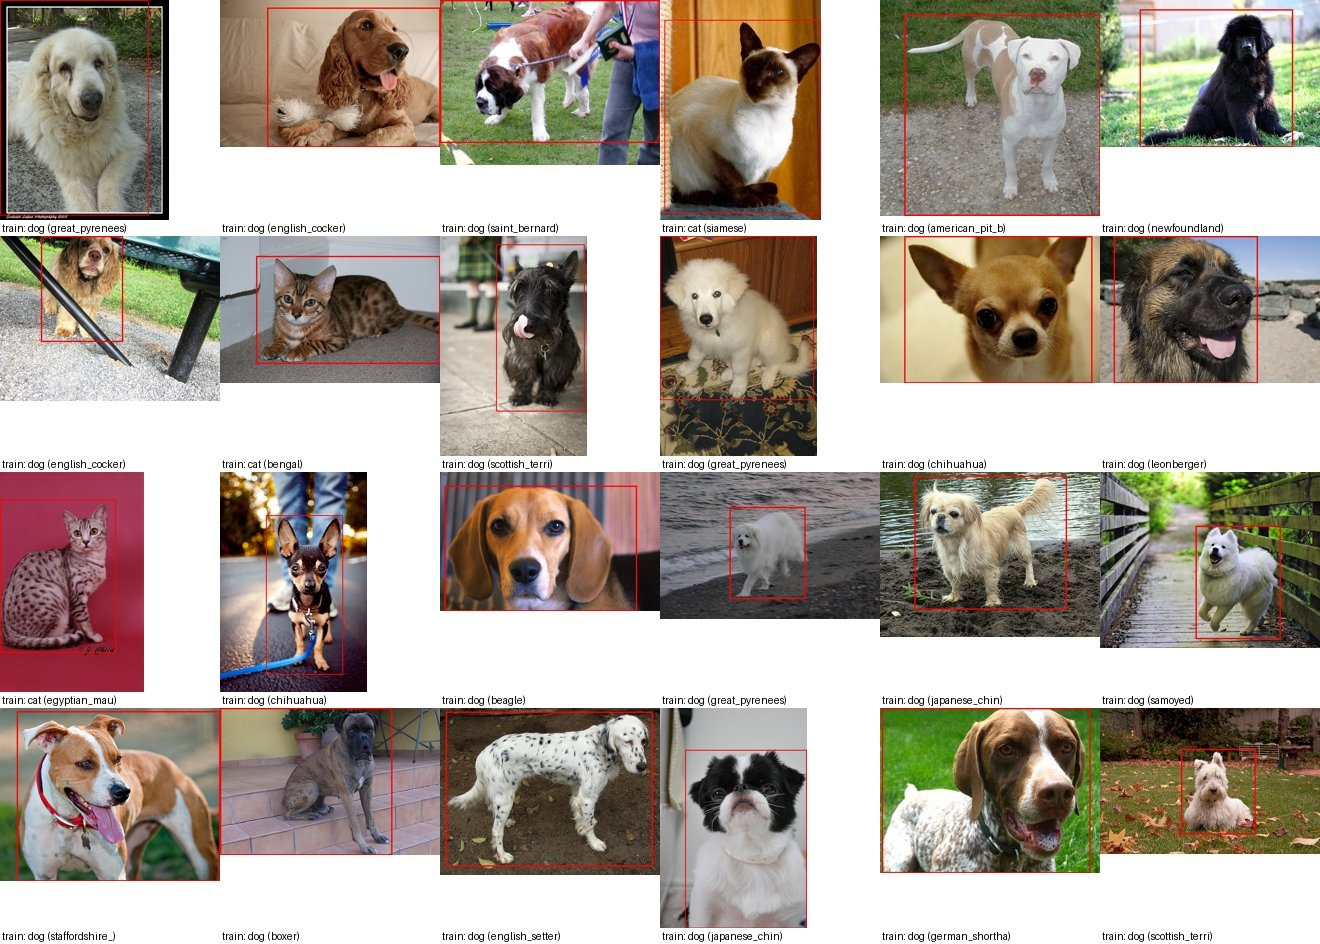
\includegraphics[width=0.78\linewidth]{figures/M4_yolo_label_check.jpg}
  \caption{Converted YOLO body boxes drawn back onto training images (Oxford train split; native resolution; no threshold).}
\end{figure}

\subsection{Fine-tuning}

{\small
\begin{tabularx}{\linewidth}{@{}l Y l Y r r@{}}
\toprule
Run (W\&B link) & Model and pretrained weights & Input res. & What changed in this run & Val.\ mAP50 & Val.\ mAP50--95 \\
\midrule
\run{48vh56vh} & YOLO11s, COCO & 640\,px & Baseline settings: 40 epochs, batch 16, SGD (auto), lr0 0.01, mosaic (off for last 10 epochs), horizontal flip 0.5, scale 0.5, HSV jitter, seed 42 & 0.979 & 0.844 \\
\run{2seovilv} & YOLO11s, COCO & 640\,px & Same settings, full rerun on 18--19 October to check reproducibility & 0.979 & 0.844 \\
\bottomrule
\end{tabularx}}

\smallskip
\textbf{Selected model and why:} the \run{2seovilv} checkpoint (the rerun reproduced every metric of the first run). Validation mAP50 was already 0.979 with the default recipe, so no further variants were trained; this means the effect of other settings is not measured. Augmentations: horizontal flips and scale changes match pets photographed from either side at different distances; vertical flips are off because pets are rarely upside down; mosaic is switched off for the last 10 epochs so the model ends on whole images like the deployment input.

\begin{figure}[H]
  \centering
  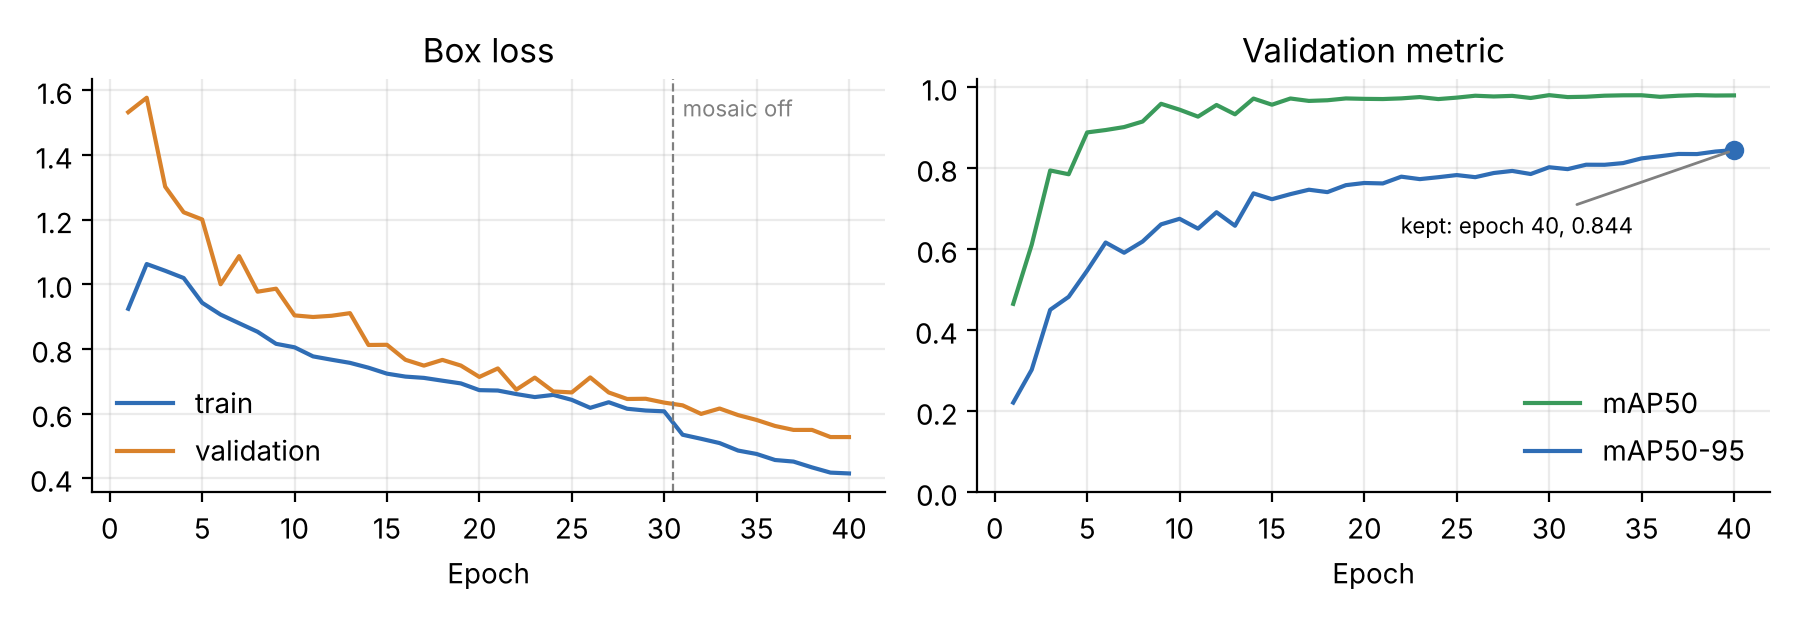
\includegraphics[width=0.9\linewidth]{figures/M4_training_curves.png}
  \caption{Run \run{2seovilv}: box loss (train and validation) and validation mAP (Oxford train/validation splits, 640\,px, evaluation \tconf{} 0.001). Validation loss still falls at epoch 40, so there is no sign of over-fitting; the drop at epoch 31 is mosaic being switched off. The kept checkpoint (\texttt{best.pt}, Ultralytics fitness $0.1\,\text{mAP50}+0.9\,\text{mAP50--95}$) is epoch 40.}
\end{figure}

\subsection{Threshold sweep and operating point}

The sweep covered \tconf{} 0.05--0.70 and \tnms{} 0.50, 0.60, 0.70 on the validation split (24 settings). The best F1 at \tnms{} 0.60 and 0.70 was 0.9576 and 0.9546, below 0.9579 at 0.50, so \tnms{} 0.50 was kept. The table shows \tnms{} 0.50.

\begin{tabularx}{\linewidth}{@{}Y Y r r r@{}}
\toprule
\tconf & \tnms & Precision & Recall & F1 \\
\midrule
0.05 & 0.50 & 0.827 & 0.992 & 0.902 \\
0.20 & 0.50 & 0.937 & 0.965 & 0.951 \\
0.30 & 0.50 & 0.955 & 0.960 & 0.958 \\
0.50 & 0.50 & 0.965 & 0.950 & 0.958 \\
0.70 & 0.50 & 0.972 & 0.905 & 0.937 \\
\midrule
\textbf{Selected: 0.40} & \textbf{0.50} & \textbf{0.959} & \textbf{0.957} & \textbf{0.958} \\
\bottomrule
\end{tabularx}

\begin{figure}[H]
  \centering
  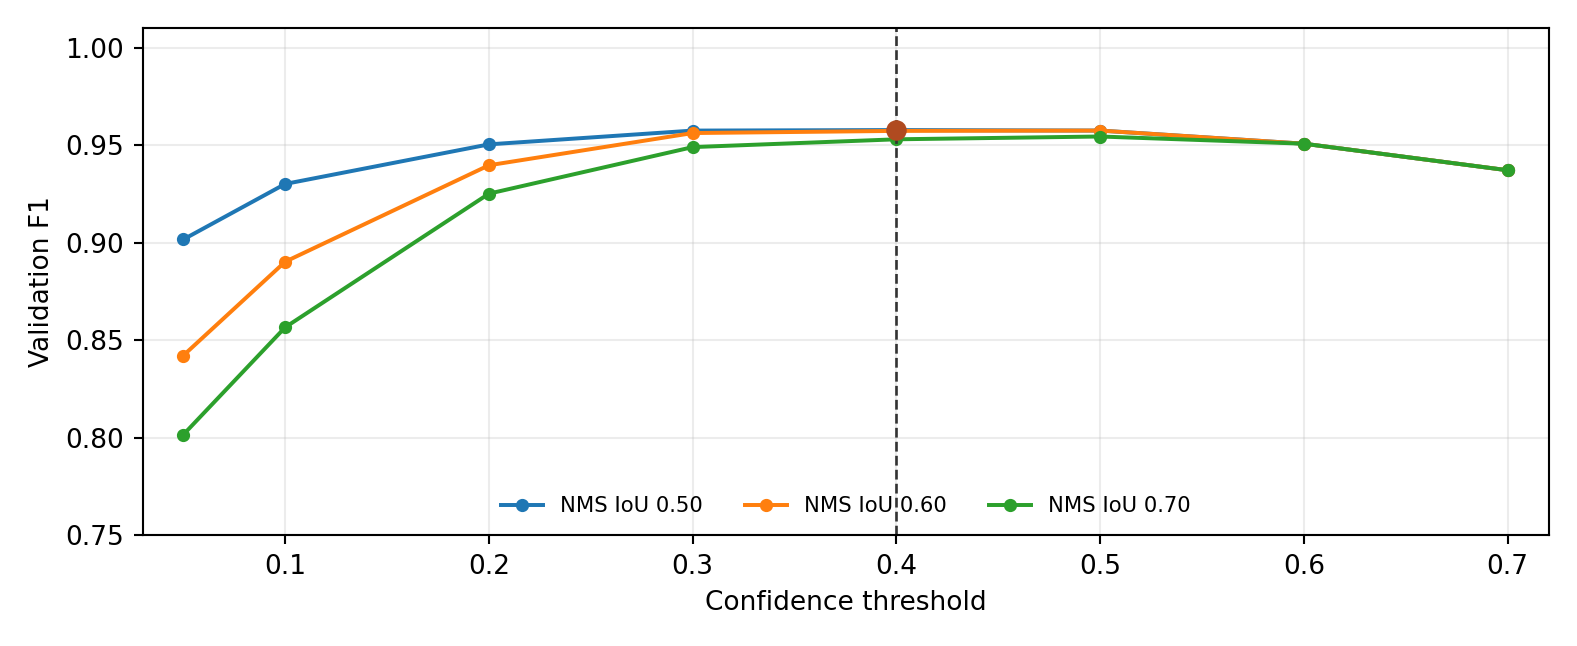
\includegraphics[width=0.78\linewidth]{figures/M4_threshold_sweep.png}
  \caption{Precision, recall and F1 against \tconf{} on the validation split (1,106 images; 640\,px; \tnms{} 0.50--0.70; selected \tconf{} 0.40, \tnms{} 0.50).}
\end{figure}

\textbf{Justification of the operating point:} the rule is the highest F1 with validation recall $\geq0.80$ (criterion A4). Both error types matter here: a missed animal hides a second pet from the count, while a false box causes an unnecessary referral. F1 is flat between \tconf{} 0.30 and 0.50 (0.958), so the choice is stable; the referral rule and the mandatory staff approval absorb the remaining errors.

\subsection{Test results}

mAP is measured by Ultralytics validation at \tconf{} 0.001; precision, recall and F1 at the operating point (\tconf{} 0.40, \tnms{} 0.50), matching IoU 0.50. Oxford test split, 640\,px.

{\small
\begin{tabularx}{\linewidth}{@{}Y r r r r r r@{}}
\toprule
Class & Instances & AP50 & AP50--95 & P @ op. & R @ op. & F1 @ op. \\
\midrule
Cat & 357 & 0.994 & 0.888 & 0.980 & 0.983 & 0.982 \\
Dog & 749 & 0.973 & 0.812 & 0.948 & 0.948 & 0.948 \\
\midrule
\textbf{All classes} & \textbf{1,106} & \textbf{0.984} & \textbf{0.850} & \textbf{0.958} & \textbf{0.959} & \textbf{0.959} \\
\bottomrule
\end{tabularx}}

\smallskip
Wilson 95\% intervals from the counts (1,061 TP, 46 FP, 45 FN): precision 0.945--0.969, recall 0.946--0.969. On the team photos the recall interval is 0.691--0.768 (368 of 503 animals).

\smallskip
\textbf{Weak classes:} dog is weaker (AP50--95 0.812 vs 0.888). Dogs vary more in body shape and pose, long-bodied breeds give looser boxes, and 10 of the 46 false positives are dogs predicted as cats or the reverse. More varied dog poses and the clothed-pet images from the Phase 1 plan would help most.

\medskip
Recall by object size. Size bins are the box area as a share of the frame (large $\geq10\%$, medium 1--10\%, small $<1\%$), because Oxford boxes are almost all large; in COCO pixel bins at 640\,px all 1,106 test boxes and all 503 team boxes are ``large''.

\begin{tabularx}{\linewidth}{@{}Y r r r r@{}}
\toprule
Object size (share of frame) & Oxford test & Recall @ op. & Team photos & Recall @ op. \\
\midrule
Small ($<1\%$) & 0 & -- & 10 & 0.000 \\
Medium (1--10\%) & 1 & 1.000 & 89 & 0.169 \\
Large ($\geq10\%$) & 1,105 & 0.959 & 404 & 0.874 \\
\bottomrule
\end{tabularx}

\subsection{Error analysis}

Oxford test split, operating point (\tconf{} 0.40, \tnms{} 0.50), matching IoU 0.50. Types follow \texttt{detect.py}: a false positive is classed by its best IoU with any ground-truth box.

\begin{tabularx}{\linewidth}{@{}l Y r r@{}}
\toprule
Type & Definition & Count & Share (\%) \\
\midrule
Duplicate & IoU $\geq0.5$ with an already matched box of the same class & 0 & 0.0 \\
Classification & IoU $\geq0.5$ with a box of the other species & 10 & 21.7 \\
Localisation & Same species, $0.1\leq$ IoU $<0.5$ & 34 & 73.9 \\
Localisation and class & Other species, $0.1\leq$ IoU $<0.5$ & 1 & 2.2 \\
Background & IoU $<0.1$ with every box & 1 & 2.2 \\
\midrule
Missed (FN) & 45 animals: 34 with a displaced box, 4 with the wrong species, 7 with no box at all & 45 & -- \\
\bottomrule
\end{tabularx}

\begin{figure}[H]
  \centering
  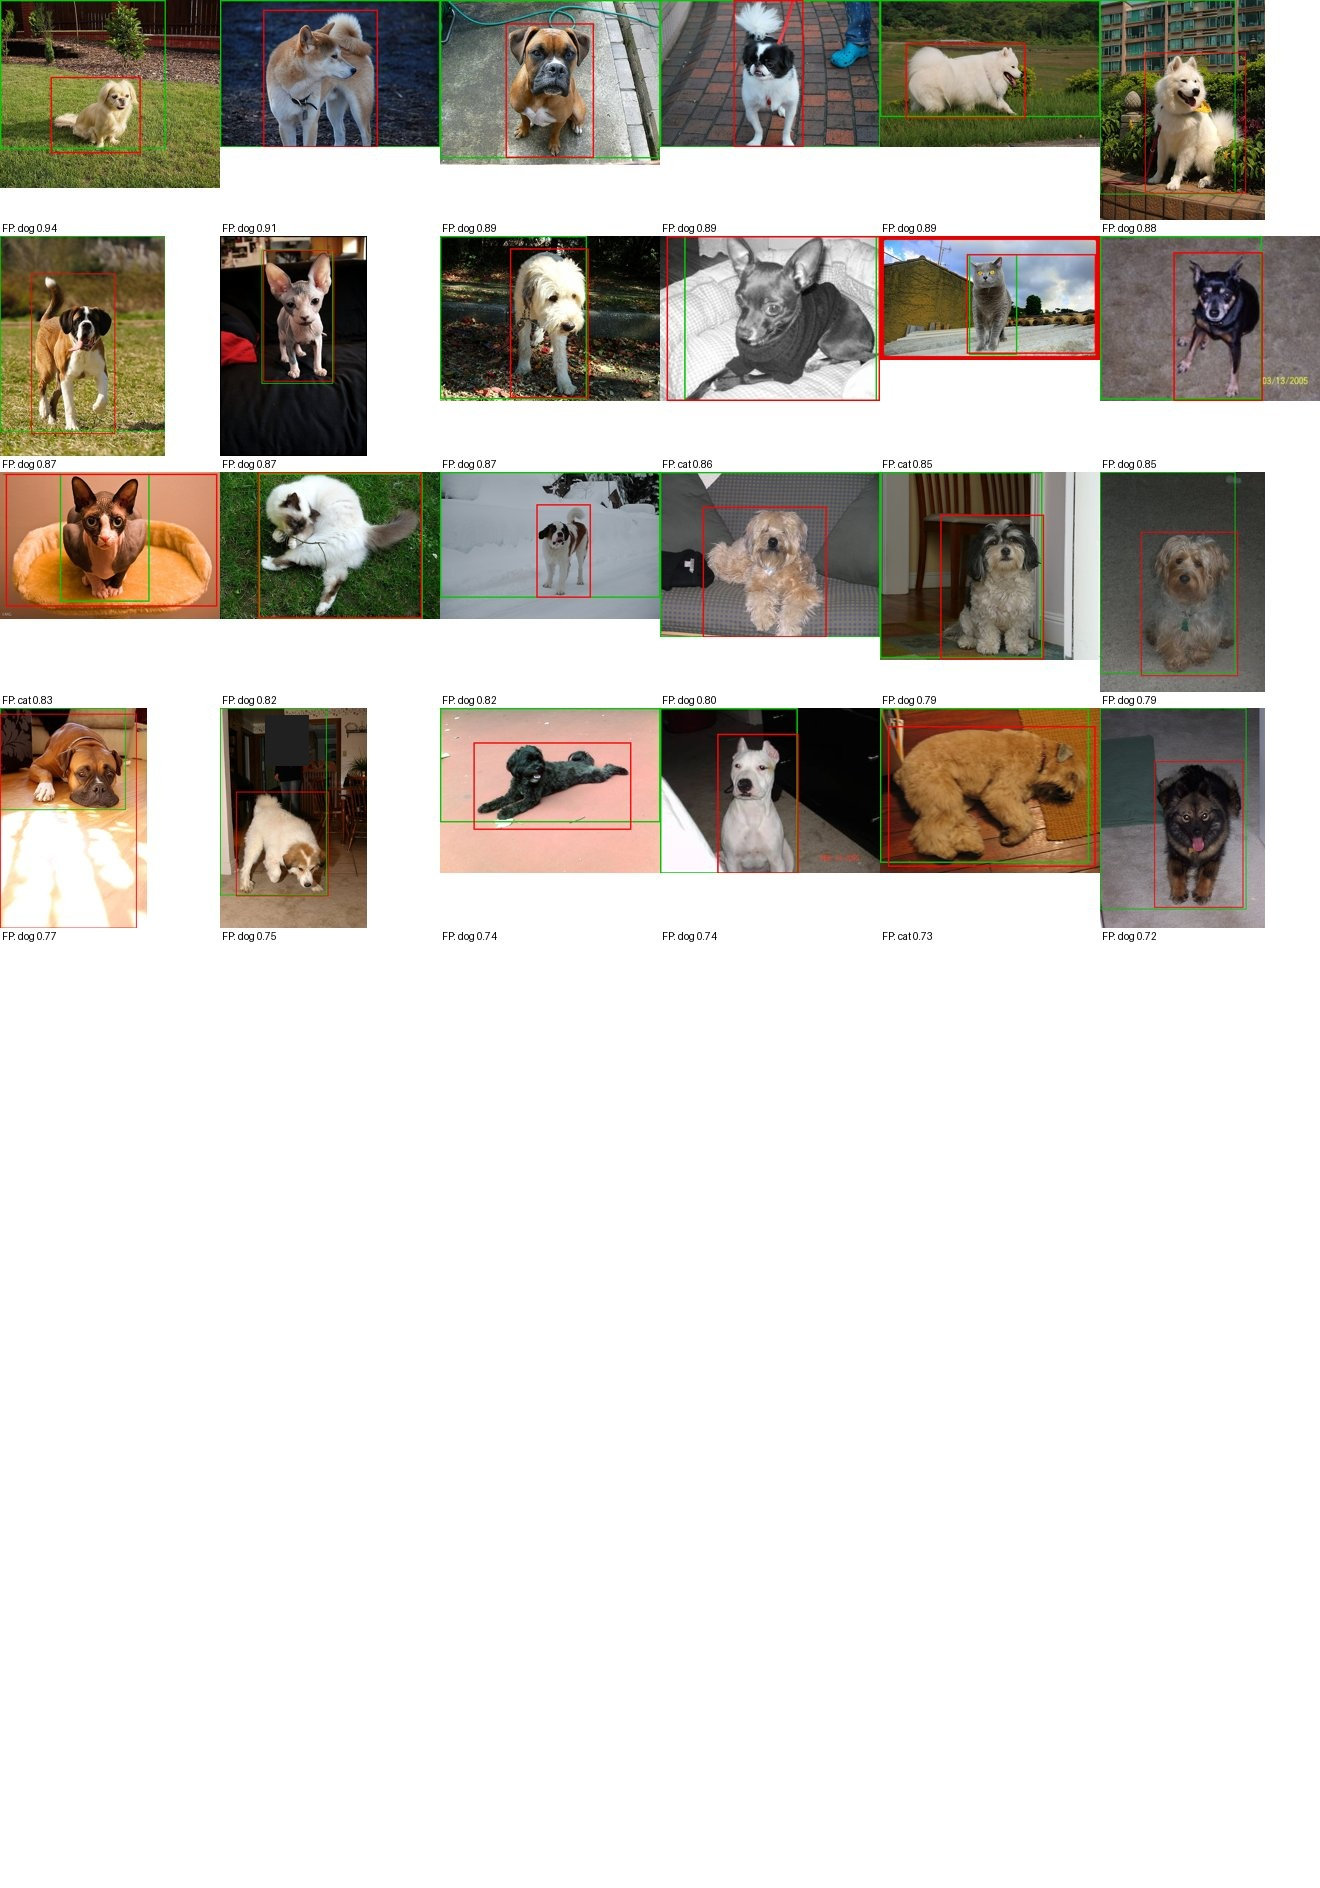
\includegraphics[width=0.48\linewidth]{figures/M4_false_positives_gallery.jpg}\hfill
  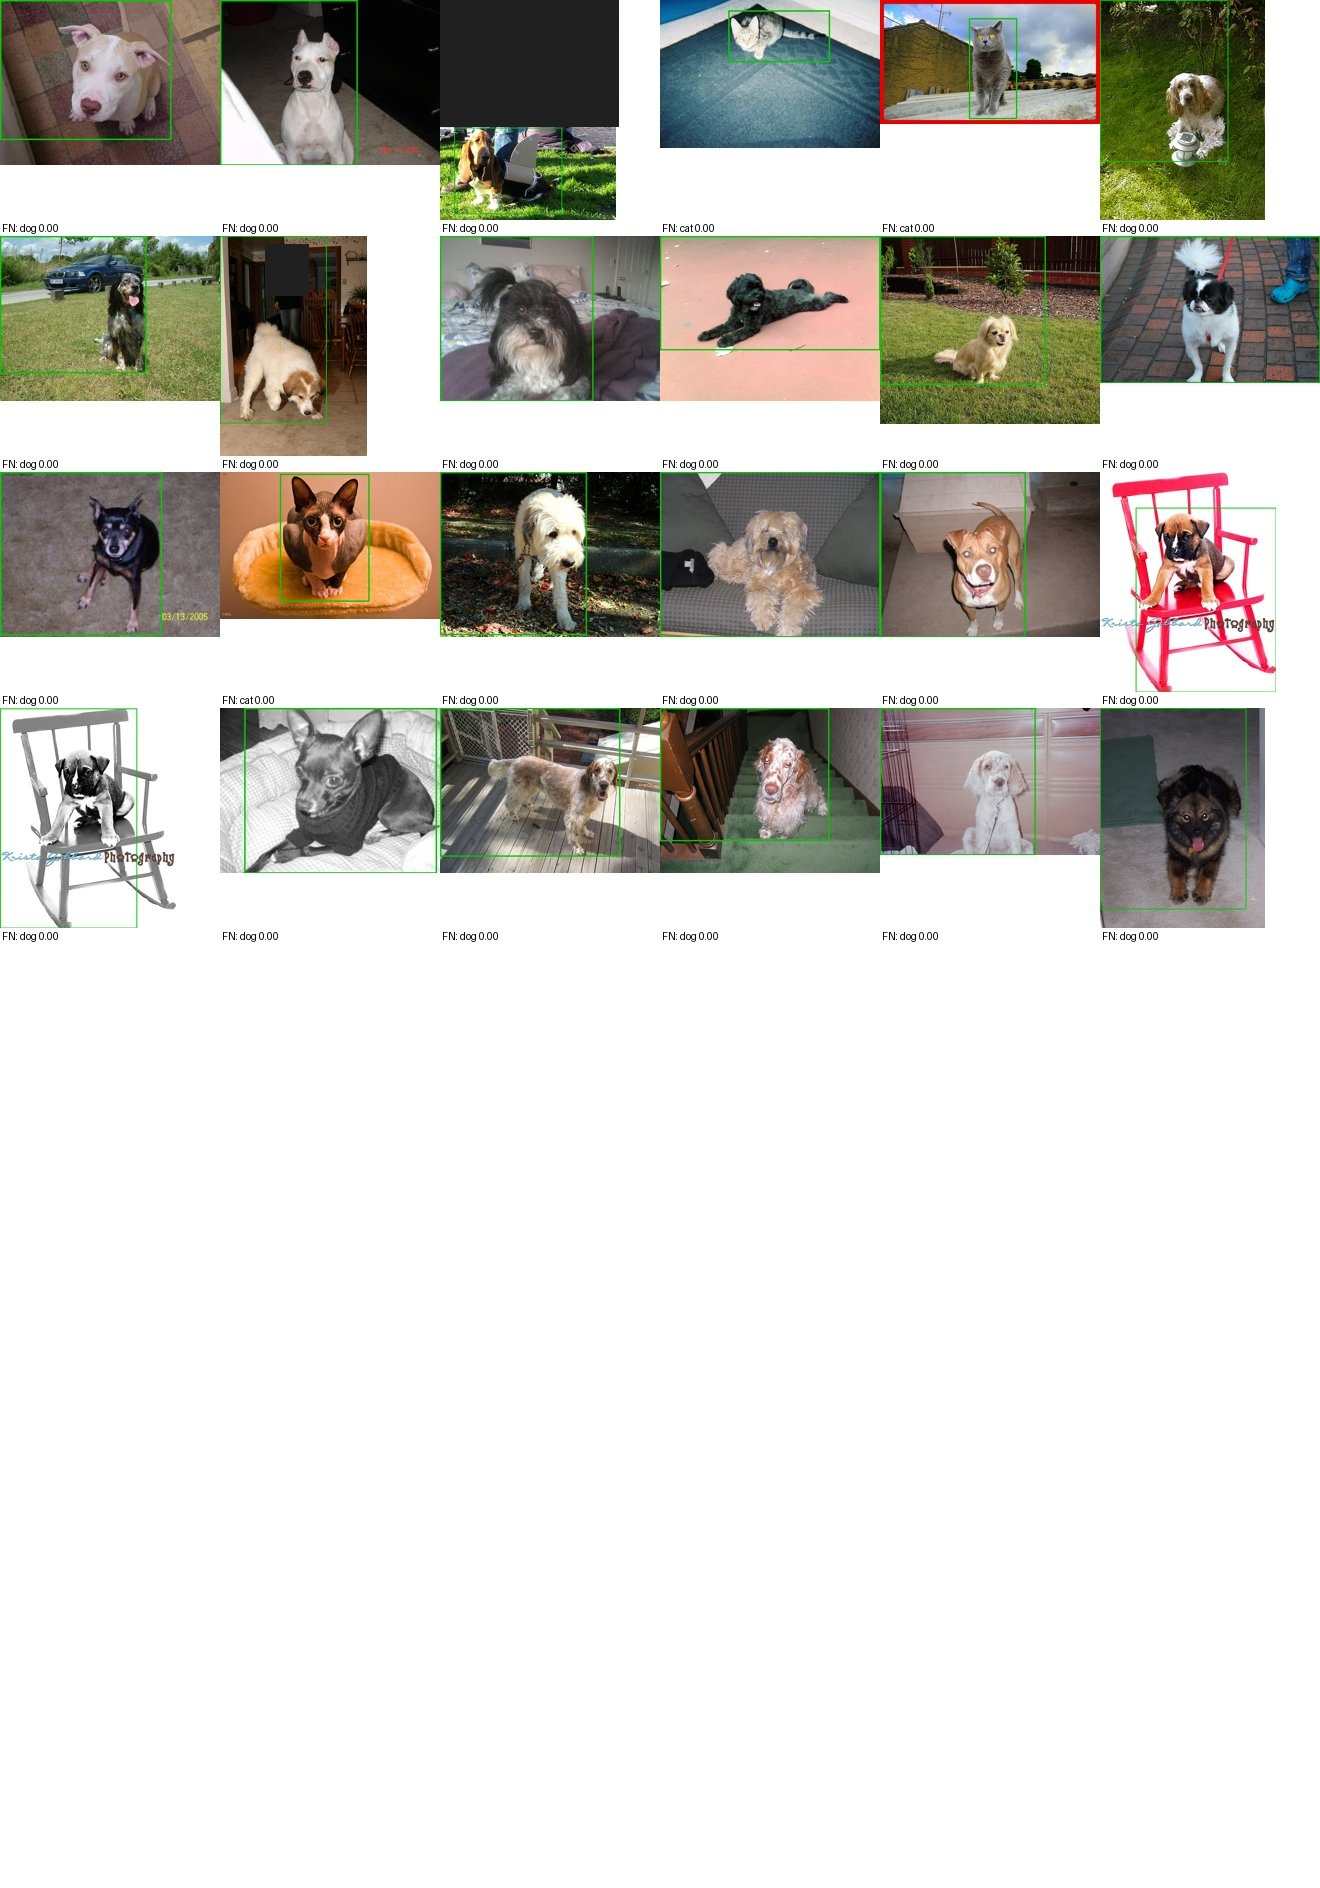
\includegraphics[width=0.48\linewidth]{figures/M4_false_negatives_gallery.jpg}
  \caption{(Left) false positives; (right) false negatives (Oxford test split; 640\,px; \tconf{} 0.40, \tnms{} 0.50; matching IoU 0.50).}
\end{figure}

\textbf{Main causes of false negatives:} 38 of the 45 are in images that also have a false positive: the box was found but displaced, mostly for curled-up or partly hidden animals and loose trimap boundaries. Only 7 animals had no detection at all.

\textbf{Failure case:} a dark Chihuahua wearing clothing (\texttt{chihuahua\_156}) was detected as a cat. The clothing hides the body outline that separates small dogs from cats. In the system the classifier returned ``dog'', so the photo was referred for disagreement; more clothed-pet training images would fix the detector itself.

\textbf{Next fix:} localisation (34 of 46 false positives and 34 of 45 misses). Re-deriving loose body boxes and adding curled-up and occluded animals to training addresses the largest error source; on shelter photos the larger gap is small and secondary animals (recall 0.000 and 0.169 in the small and medium bins).

\subsection{Inference on images and video}\label{sec:team}

\textbf{Team photos.} The 401 team photos (503 annotated animals, never used for training or selection) were run at the same operating point: mAP50 0.771, mAP50--95 0.653; precision 0.885, recall 0.732, F1 0.801; cat recall 0.854, dog recall 0.651. The animal count was correct on 339 of 401 photos, and in only 11 of 52 multi-animal photos were all animals found.

\begin{figure}[H]
  \centering
  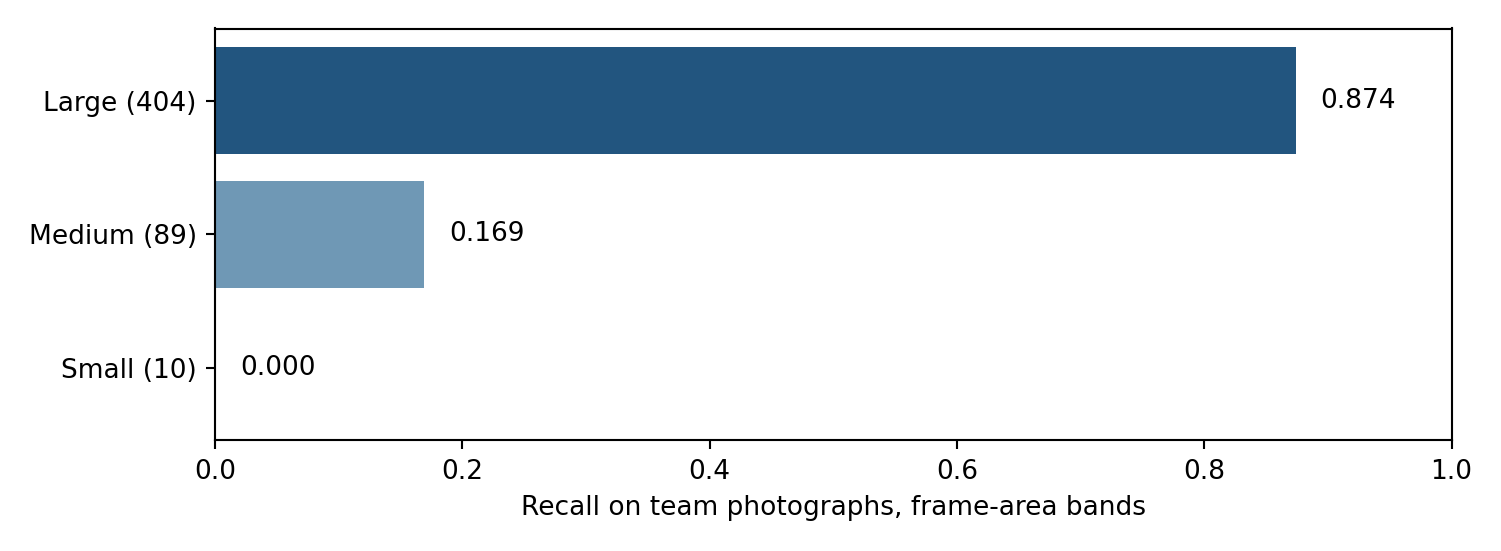
\includegraphics[width=0.78\linewidth]{figures/M4_size_recall.png}
  \caption{Recall by animal size on the team photos (401 photos, 503 animals; 640\,px; \tconf{} 0.40, \tnms{} 0.50).}
\end{figure}

\textbf{Video.} Two openly licensed Wikimedia Commons clips were processed frame by frame on a Tesla T4 at 640\,px, \tconf{} 0.40, \tnms{} 0.50, batch 1.

{\small
\begin{tabularx}{\linewidth}{@{}Y r r r Y@{}}
\toprule
Clip (licence) & Frames & Mean / p95 (ms) & FPS & Frames with 0 / 1 / 2+ boxes; labels \\
\midrule
Africanis Dogs Resting in Grass (CC0) & 506 & 12.0 / 14.2 & 83.4 & 0 / 506 / 0; all dog \\
Cat in a Bag (CC BY 2.0) & 510 & 11.3 / 14.6 & 88.4 & 222 / 286 / 2; 286 cat, 4 dog \\
\bottomrule
\end{tabularx}}

\begin{figure}[H]
  \centering
  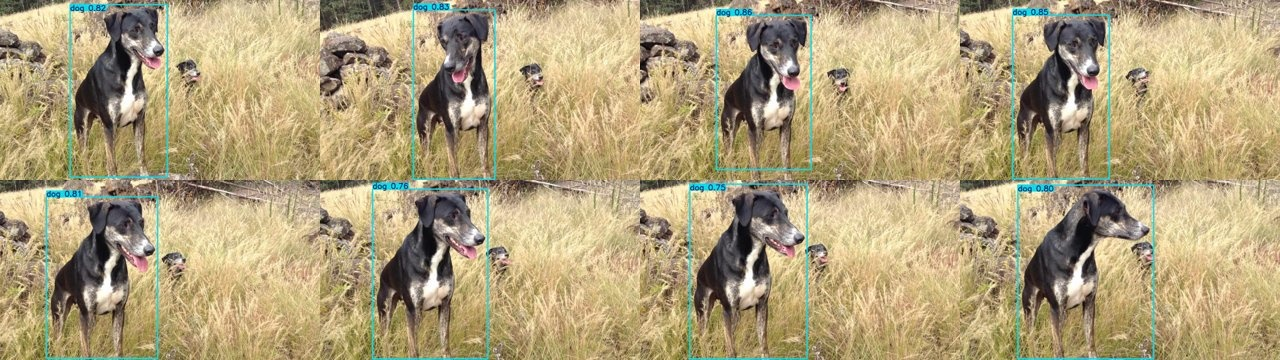
\includegraphics[width=0.88\linewidth]{figures/M4_video_Africanis_Dogs_Resting_In_Grass.jpg}\\[3pt]
  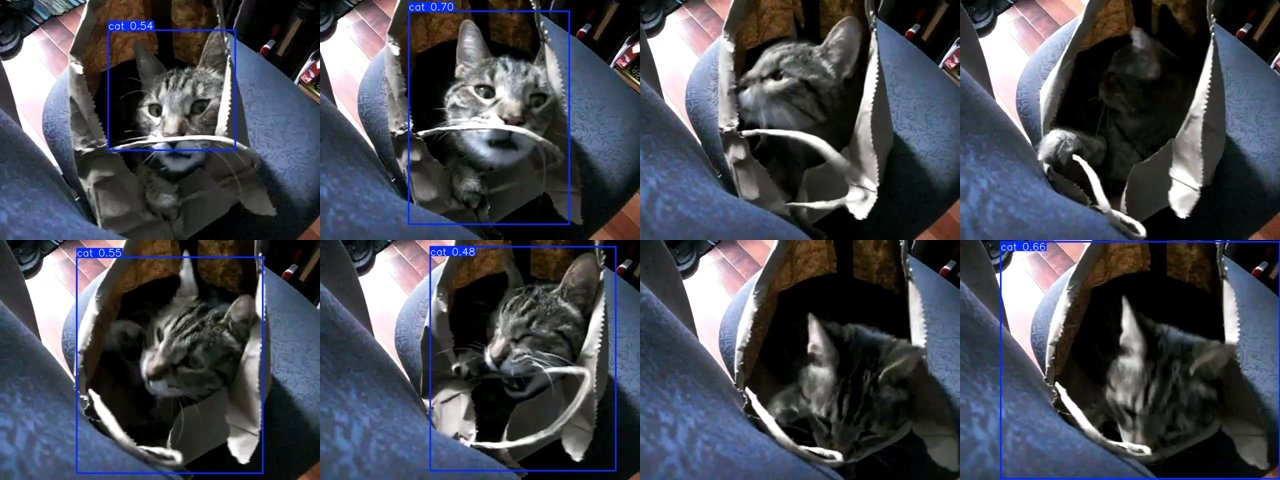
\includegraphics[width=0.88\linewidth]{figures/M4_video_Cat_in_a_Bag.jpg}
  \caption{Detector frames from the two clips (external licensed video; 640\,px; \tconf{} 0.40, \tnms{} 0.50; T4). The cat is hidden behind the bag in most of the 222 frames without a box; 4 frames label it as a dog.}
\end{figure}

% =====================================================================
\section{Segmentation (M5)\pts{15}{12}}

\textbf{Task:} instance segmentation of the animal's whole body (classes cat, dog). The mask is matched to the animal selected by the detector: no matching mask, a mask share of the image below 0.05, a second animal or a species different from the detector's all trigger a referral. Instance segmentation fits because a shelter photo can contain several animals and the rule needs one mask per animal, not a single foreground map.

The checkpoint was chosen on validation; the mask confidence and matching settings were set once (Section 3.3); the test split was evaluated once.

\subsection{Ground-truth masks}

\begin{tabularx}{\linewidth}{@{}l Y@{}}
\toprule
Item & Our answer \\
\midrule
Source of masks & Oxford-IIIT Pet pixel trimaps: body mask = foreground plus the ambiguous border class. SAM 2.1-B, prompted with the ground-truth box, produced a second set of 300 test masks used as the baseline \\
Images with masks (train / val / test) & 5,123 / 1,106 / 1,106 \\
Class distribution & One animal per image: cat 1,652 / 357 / 357; dog 3,471 / 749 / 749 \\
How masks were checked & Automatic: images without a usable trimap removed in cleaning; visual: a gallery of test masks overlaid on the images (Figure~\ref{fig:gtmask}) and the 300 SAM masks, by the segmentation workstream \\
Masks corrected or rejected & 14 images rejected for an empty trimap (Phase 1 cleaning); no mask was hand-edited \\
Label format & YOLO segmentation polygons from the binary body mask. Border pixels count as body in the main metric; a second metric ignores them \\
\bottomrule
\end{tabularx}

\begin{figure}[H]
  \centering
  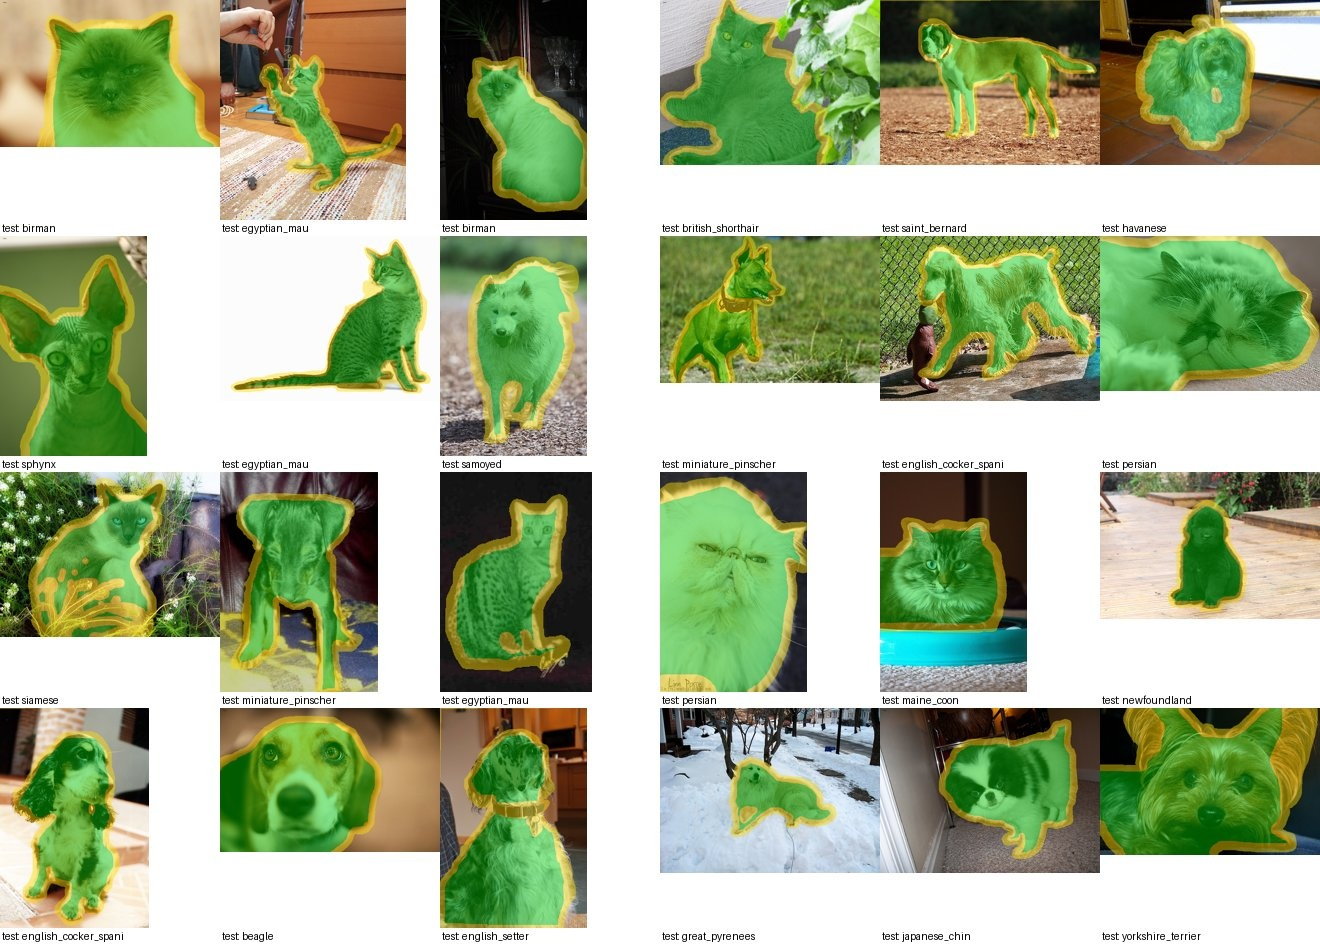
\includegraphics[width=0.78\linewidth]{figures/M5_gt_mask_check.jpg}
  \caption{Ground-truth body masks (trimap foreground plus border) overlaid on Oxford test images (native resolution; binary mask, no threshold).}\label{fig:gtmask}
\end{figure}

\subsection{Model and training}

The baseline is SAM 2.1-B used as is, prompted with the ground-truth box (an oracle prompt, so it shows how good masks can be without any training). The fine-tuned model is YOLO11s-seg, which finds the animal by itself.

{\small
\begin{tabularx}{\linewidth}{@{}p{2.1cm} p{2.3cm} p{1.5cm} X p{1.0cm} p{2.2cm}@{}}
\toprule
Run (W\&B) & Model and initial weights & Train / eval res. & Training setup (loss, augmentation, optimiser) & Epochs & Val.\ metric \\
\midrule
Baseline \run{1jb5y453} & SAM 2.1-B, released weights & -- / native & No training; prompt = ground-truth box & -- & Not run on val (test 300: mIoU 0.812) \\
\run{kd5ksgt3} & YOLO11s-seg, COCO & 640 / 640\,px & Box, class, DFL and mask losses; mosaic (off last 10 epochs), flip 0.5, scale 0.5, HSV; SGD (auto), lr0 0.01, batch 16, seed 42 & 40 & mask mAP50--95 0.878 \\
\run{3ztpz2tc} & YOLO11s-seg, COCO & 640 / 640\,px & Same settings, full rerun (18--19 October) & 40 & mask mAP50--95 0.878 \\
\bottomrule
\end{tabularx}}

\smallskip
\textbf{Selected run and why (chosen on validation):} \run{3ztpz2tc}: validation mask mAP50 0.993 and mAP50--95 0.878, identical to the first run, so the recipe is reproducible. No other recipe was trained.

\begin{figure}[H]
  \centering
  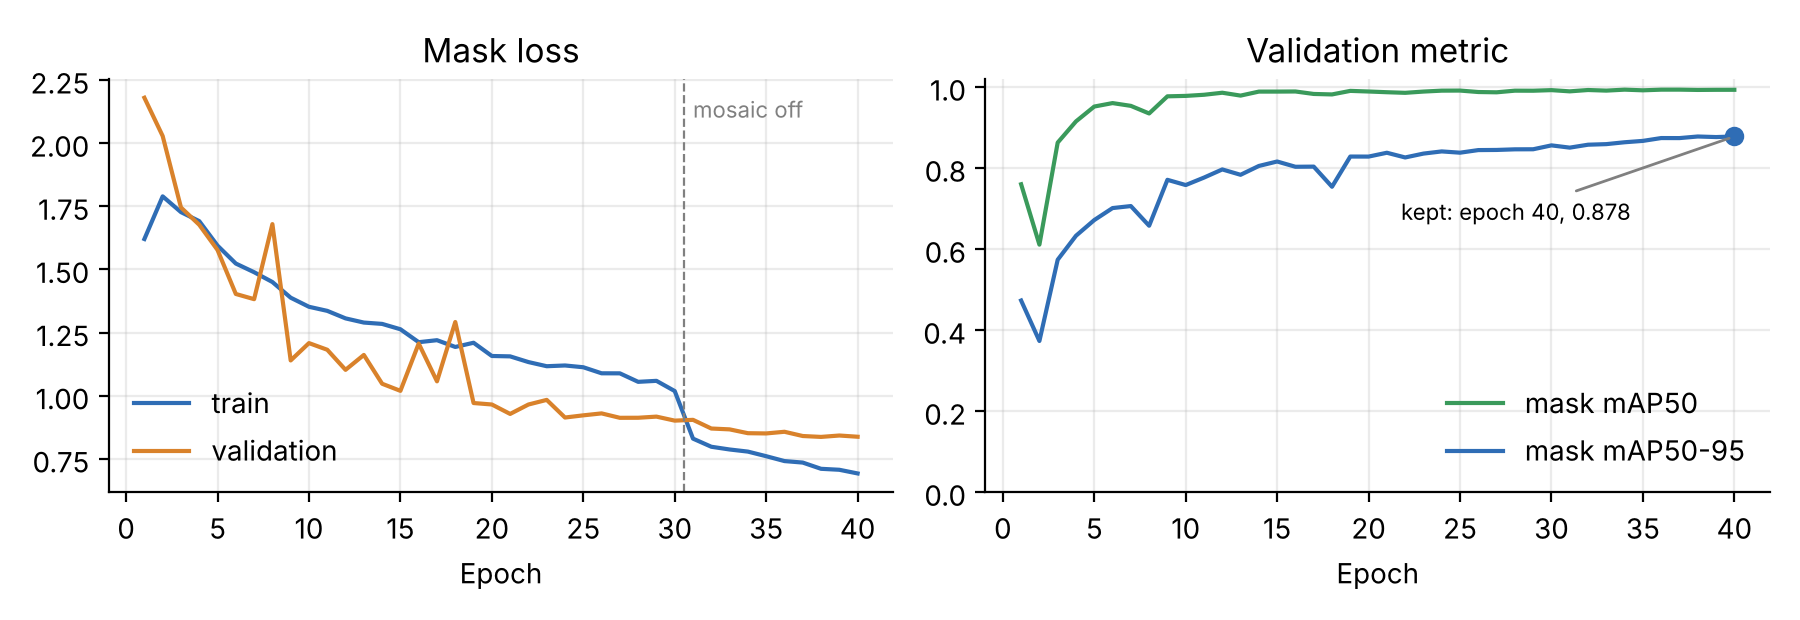
\includegraphics[width=0.9\linewidth]{figures/M5_training_curves.png}
  \caption{Run \run{3ztpz2tc}: mask loss (train and validation) and validation mask mAP (Oxford train/validation splits; 640\,px; evaluation \tconf{} 0.001). Validation loss flattens after epoch 32 without rising; the drop at epoch 31 is mosaic being switched off. The kept checkpoint (\texttt{best.pt}) is epoch 40.}
\end{figure}

\subsection{Thresholds and post-processing}

These settings were set once in the configuration and were not swept on validation; this is a gap in our protocol.

\begin{tabularx}{\linewidth}{@{}l Y l l@{}}
\toprule
Setting & Values tried & Validation metric & Chosen \\
\midrule
Mask confidence (YOLO) & 0.25 only (Ultralytics default) & Not swept & 0.25 \\
Mask-to-box match IoU & 0.10 only & Not swept & 0.10 \\
Minimum mask share of the image & 0.05 only & Not swept & 0.05 \\
Mask resolution & \texttt{retina\_masks=True} (full resolution) & -- & on \\
\bottomrule
\end{tabularx}

\subsection{Test results}

Mean IoU and Dice are the means of per-image binary scores on the union of all predicted instances versus the ground-truth body mask; ``no border'' excludes the trimap border pixels. Mask mAP50--95 is the class-aware Ultralytics instance metric (\tconf{} 0.001). Oxford test split, 640\,px, mask \tconf{} 0.25.

{\small
\begin{tabularx}{\linewidth}{@{}Y l r r r r@{}}
\toprule
Model & Split & Mask mAP50--95 & mIoU & Mean Dice & mIoU, no border \\
\midrule
Baseline SAM 2.1-B (oracle box) & Test, 300 sampled & -- & 0.812 & 0.883 & 0.948 \\
Selected run, same 300 images & Test, 300 sampled & -- & 0.925 & 0.960 & 0.934 \\
Selected run & Val & 0.878 & -- & -- & -- \\
Selected run & Test, all 1,106 & 0.875 & 0.923 & 0.959 & 0.930 \\
\bottomrule
\end{tabularx}}

\medskip
\begin{tabularx}{\linewidth}{@{}Y r r r@{}}
\toprule
Class (test, 1,106) & IoU & Dice & Mask AP \\
\midrule
Cat (357) & 0.929 & 0.962 & not recorded per class \\
Dog (749) & 0.920 & 0.957 & not recorded per class \\
\bottomrule
\end{tabularx}

\begin{figure}[H]
  \centering
  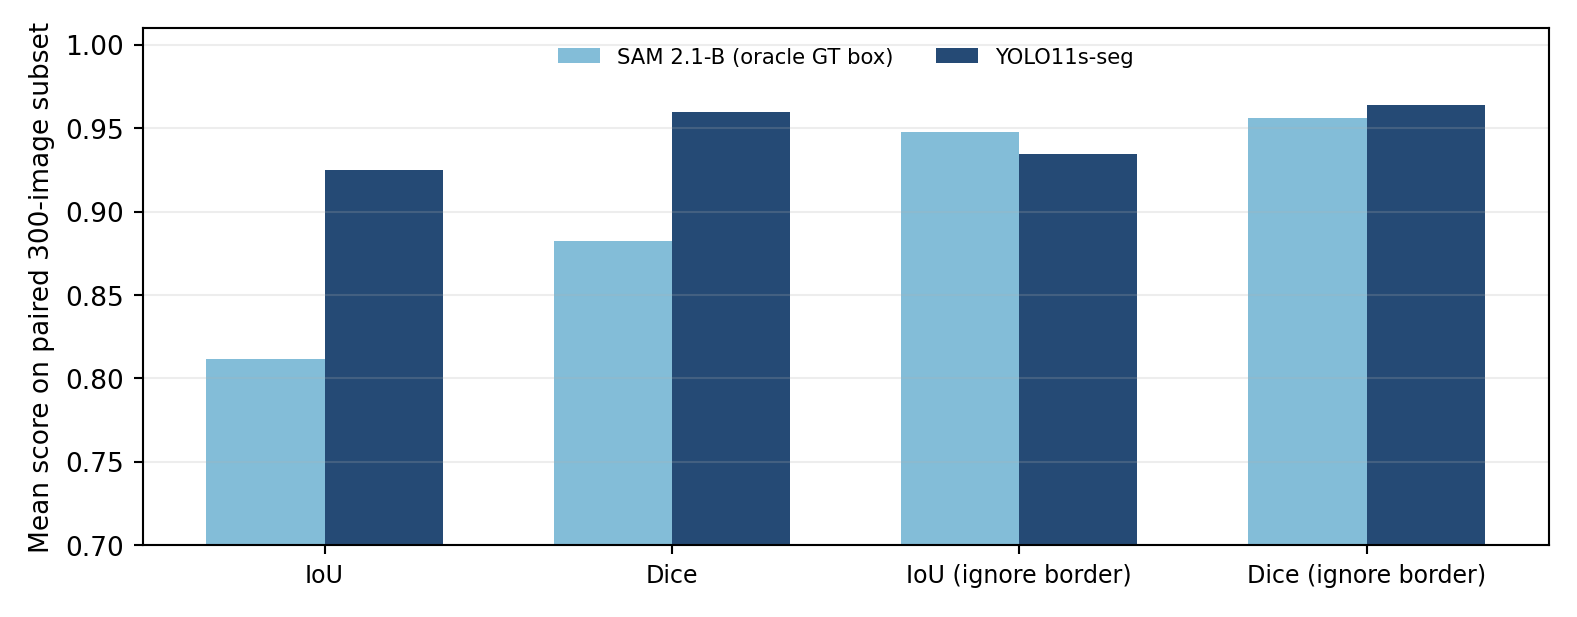
\includegraphics[width=0.85\linewidth]{figures/M5_paired_metrics.png}
  \caption{Mean IoU and Dice on the same 300 test images for the SAM 2.1-B baseline (native resolution, ground-truth box prompt) and YOLO11s-seg (640\,px, \tconf{} 0.25), with and without trimap border pixels.}
\end{figure}

\textbf{Application measure:} on the 401 team photos (CPU run \run{f8manl0i}, 640\,px, \tconf{} 0.25), the number of segmented animals equals the annotated number on 355 of 401 photos (88.5\%), and the mask's species agrees with the true label on 372 of 378 single-species photos with a mask. Masks triggered 30 referral reasons: 13 animal too small, 10 species disagreement, 7 no matching mask. On Oxford test, fine-tuning raises mean IoU from 0.812 (SAM with an oracle box) to 0.925 on the same 300 images; with border pixels ignored SAM is higher (0.948 vs 0.934), so most of SAM's gap is the trimap border convention rather than wrong masks.

\subsection{Error analysis}

\begin{figure}[H]
  \centering
  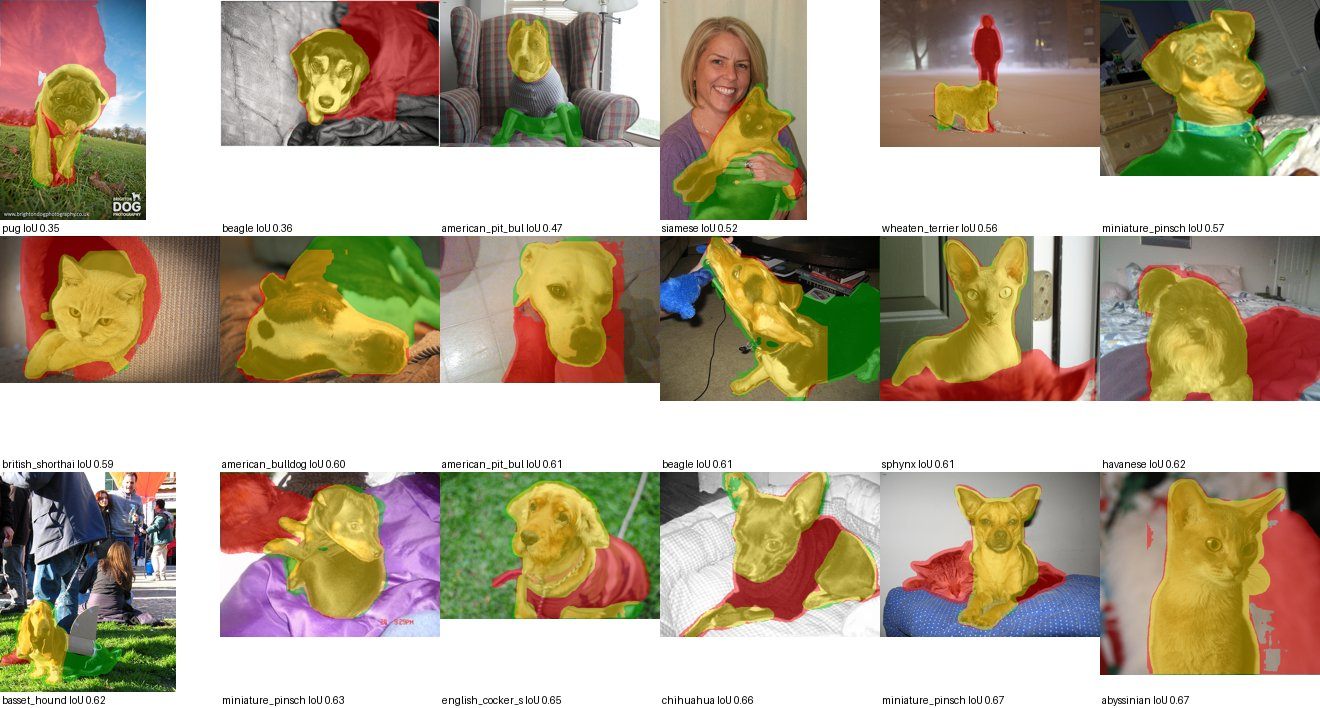
\includegraphics[width=0.95\linewidth]{figures/M5_yolo_seg_failures.jpg}
  \caption{The 18 lowest-IoU YOLO11s-seg predictions on the Oxford test split (640\,px, \tconf{} 0.25). Yellow: prediction and ground truth agree; red: prediction only; green: ground truth only.}
\end{figure}

\begin{tabularx}{\linewidth}{@{}Y l Y@{}}
\toprule
Error pattern & Examples & Likely cause \\
\midrule
Mask spreads into a blanket, cushion or clothing of similar colour & british\_shorthair 0.59, havanese 0.62, chihuahua 0.66 & Weak colour boundary; trimap border included in training targets \\
Part of the body missed (green) & beagle 0.36, american\_pit\_bull 0.47 & Occlusion by furniture or a person; dark fur on dark background \\
Mask covers a person or a second object & wheaten\_terrier 0.56, siamese 0.52 & Person holding or standing next to the animal \\
SAM baseline masks the background & Close-ups where the box fills the frame (Figure~\ref{fig:samfail}) & Oracle box gives no inside/outside cue; 12 of 300 SAM masks have IoU $<0.5$ \\
\bottomrule
\end{tabularx}

\begin{figure}[H]
  \centering
  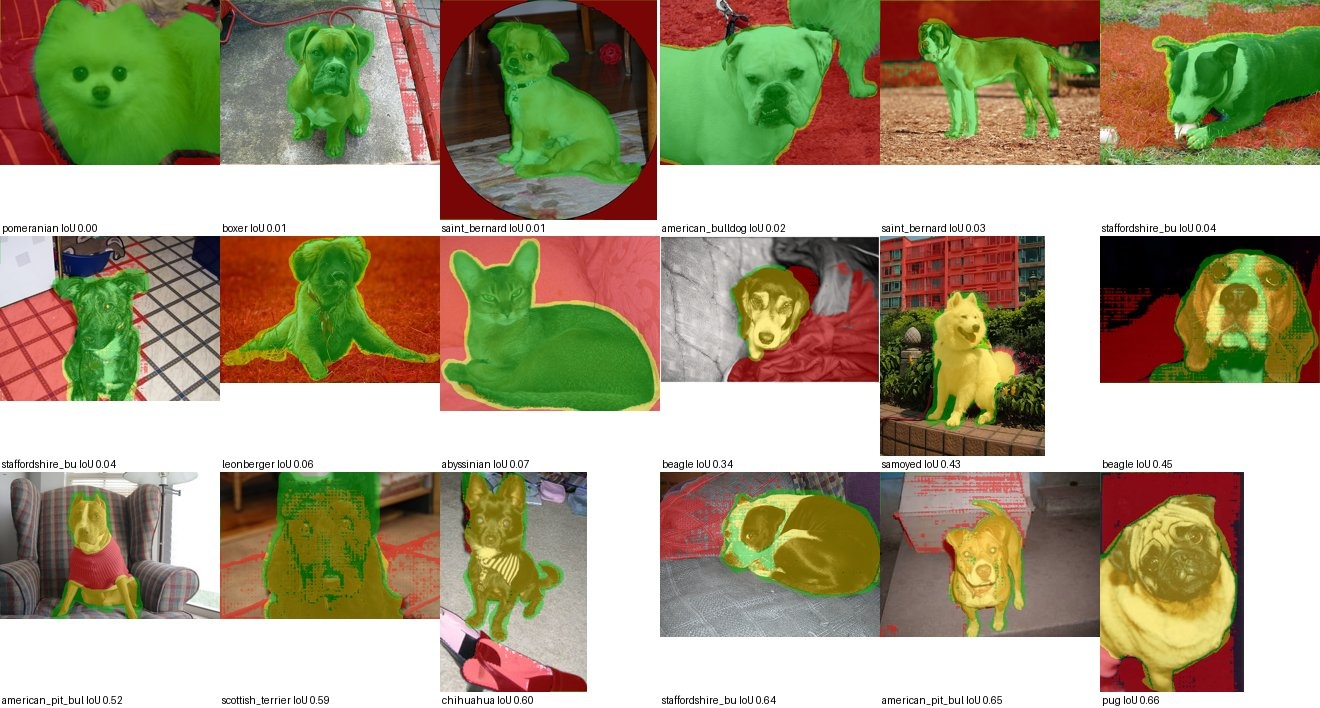
\includegraphics[width=0.78\linewidth]{figures/M5_sam_baseline_failures.jpg}
  \caption{Lowest-IoU SAM 2.1-B baseline masks (Oxford test, 300 sampled; native resolution; ground-truth box prompt).}\label{fig:samfail}
\end{figure}

\textbf{Failure case:} the pug image (IoU 0.35): the model masked the dog but also a large patch of sky (red), probably because the bright sky and the fawn coat have similar contrast to the grass. More outdoor training images and a check that the mask lies inside the detector box (the integration rule already matches masks to the box) would limit the effect on the verdict.

% =====================================================================
\section{System integration and deployment (M8)\pts{15}{11}}

Every number states its hardware and path. The acceptance benchmark (A8) is in-process on a Tesla T4; the service checks went through HTTP to a separate uvicorn process, once on the T4 and once on CPU only.

\subsection{End-to-end pipeline}

Per-stage times are means from the instrumented pipeline (\texttt{timings} in each response); per-stage percentiles were not recorded. The end-to-end time was measured directly per image.

\begin{tabularx}{\linewidth}{@{}l Y r r@{}}
\toprule
Stage & Implementation & Mean (ms) & p95 (ms) \\
\midrule
Pre-processing & PIL decode; letterbox inside Ultralytics; crop and resize for the classifier & incl.\ below & -- \\
Model inference: detector & YOLO11s, PyTorch CUDA, 640\,px & 14.2 & -- \\
Model inference: classifier & ResNet-50, PyTorch CUDA, 224\,px crop & 9.3 & -- \\
Model inference: segmenter & YOLO11s-seg, PyTorch CUDA, 640\,px & 17.6 & -- \\
Post-processing and decision & Mask matching and referral rule & incl.\ above & -- \\
\midrule
\textbf{End to end} & Measured per image & 41.5 (p50 38.5) & 61.4 \\
\bottomrule
\end{tabularx}

\smallskip
\textbf{Conditions:} Tesla T4, PyTorch 2.11.0 (CUDA), Ultralytics 8.4.182; batch 1; the first 50 Oxford test images cycled; 10 warm-up and 200 timed images; one process.

\subsection{Release and manifest}

The service reads every path and threshold from \texttt{runs/manifest.json}; \texttt{Manifest.load} rejects out-of-range values, and \texttt{tools/preflight\_release.py} checks the weight checksums before a run.

\begin{tabularx}{\linewidth}{@{}l Y@{}}
\toprule
Item & Our answer \\
\midrule
Model file(s) and checksum & Detector \texttt{best.pt} \texttt{f48e4d8e\ldots1cd4}; segmenter \texttt{best.pt} \texttt{868f3842\ldots d8ee}; classifier \texttt{finetune.pt} \texttt{22dd58d4\ldots81ba} (SHA-256, full values in the model card) \\
Class names and order & \texttt{["cat", "dog"]} (detector, segmenter and classifier) \\
Input size and pre-processing & Detector and segmenter: letterbox to 640\,px. Classifier: crop of the selected box, resize to 255\,px, centre crop 224\,px, ImageNet mean/std \\
Thresholds & Detector \tconf{} 0.40, \tnms{} 0.50; segmenter \tconf{} 0.25; temperature 0.05; verification threshold 0.90; minimum mask share 0.05 \\
Library and runtime versions & Python 3.13; torch 2.11.0; torchvision 0.26.0; ultralytics 8.4.182; onnxruntime 1.31.0; fastapi 0.141.1; uvicorn 0.54.0 (pinned in \texttt{requirements.txt}) \\
Manifest link & \href{https://github.com/Yasser-20-alhajlah/smart-pet-vision/blob/main/smart-pet-vision/phase2/report/evidence/M8_manifest.json}{\texttt{evidence/M8\_manifest.json}} (copy of \texttt{runs/manifest.json}; weights stay in private Drive) \\
\bottomrule
\end{tabularx}

\subsection{Input and output contracts}

\begin{tabularx}{\linewidth}{@{}l Y@{}}
\toprule
Contract & Our answer \\
\midrule
Input & \texttt{POST /analyze}, multipart field \texttt{file}: one image readable by PIL (JPEG, PNG, \ldots), any size up to 15\,MB and 25\,MP; converted to RGB; batch 1. Query \texttt{images=false} omits the annotated PNG \\
Output & JSON: \texttt{verdict} (\texttt{ready} / \texttt{refer\_to\_staff}), \texttt{reasons} (code and message), \texttt{species}, \texttt{confidence}, \texttt{probabilities}, \texttt{detections} (\texttt{box\_xyxy} in original-image pixels, species, score), \texttt{mask\_fraction}, \texttt{segmentation\_matched}, \texttt{timings} (ms); always \texttt{staff\_approval\_required: true} and \texttt{automatic\_publication\_allowed: false} \\
Thresholds served & Those of the manifest (above), reported by \texttt{GET /health} through the model names \\
Invalid input & Empty upload $\rightarrow$ HTTP 400; not an image $\rightarrow$ 415; over 15\,MB or 25\,MP $\rightarrow$ 413; no animal $\rightarrow$ 200 with \texttt{refer\_to\_staff} and reason \texttt{no\_animal} \\
\bottomrule
\end{tabularx}

\subsection{ONNX export and parity}

\textbf{Export settings:} opset 17, fixed input $1\times3\times640\times640$ (detector) and $1\times3\times224\times224$ (classifier), FP32. The detector graph contains the network and the decoded raw head (boxes in pixels and class scores); confidence filtering and NMS stay in our code. A re-check on 31 October tried six export and runtime settings (simplified or not, graph optimisation off/basic/all, one thread).

{\small
\begin{tabularx}{\linewidth}{@{}p{5.2cm} p{2.4cm} X l@{}}
\toprule
Check (PyTorch vs.\ ONNX) & Tolerance & Result & Pass? \\
\midrule
Classifier: max abs difference of logits (8 inputs) & $\leq 0.001$ (A9a) & $2.98\times10^{-7}$; argmax agreement 100\% & Yes \\
Detector: max abs difference of raw head (4 random inputs, seed 0, CPU) & $\leq 0.001$ (A9b) & 0.0018; re-check 0.0020; six settings 0.00198--0.00201 & \textbf{No} \\
Detector: same decisions at the operating point (50 Oxford test images, CPU) & None set in advance & 98\% same count and classes; largest box shift 28.7\,px & Reported \\
Same metric on the evaluation set & -- & Not measured & -- \\
Reduced precision (FP16 / INT8) & -- & Not used & -- \\
\bottomrule
\end{tabularx}}

\smallskip
On the same inputs a float64 PyTorch reference differs from float32 PyTorch by 0.0016 and from ONNX by 0.0012. This shows differences of this size also arise between float32 and float64 runs of the same model, but it does not isolate the cause of the ONNX gap, and the bound is not changed. Decision: the service runs the PyTorch detector.

\subsection{HTTP service}

\begin{tabularx}{\linewidth}{@{}l Y@{}}
\toprule
Item & Our answer \\
\midrule
Framework and hosting & FastAPI served by uvicorn (one worker); run locally or in a Colab runtime (no public hosting) \\
Endpoint(s) & \texttt{POST /analyze}, \texttt{GET /health}, \texttt{GET /docs} \\
Hardware & Tesla T4 (A7 check, \run{fqow5ly7}); CPU only, Colab (\run{mu2tolkg}) \\
Checks at start-up & Manifest values validated on load; \texttt{/health} loads the three models and returns their names; \texttt{preflight\_release.py} verifies files, SHA-256, thresholds and \texttt{review\_mode=off} before validation runs \\
Example request & \texttt{curl -X POST -F "file=@img.jpg" "http://127.0.0.1:8000/analyze?images=false"} \\
\bottomrule
\end{tabularx}

\begin{figure}[H]
  \centering
  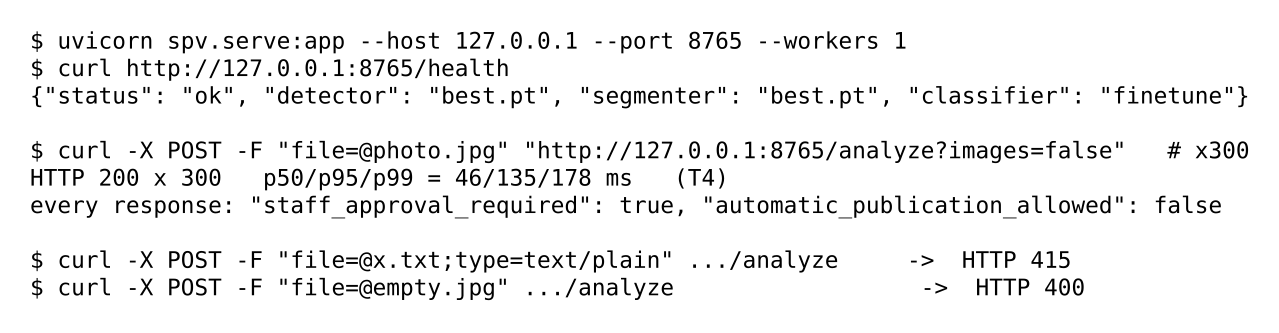
\includegraphics[width=0.85\linewidth]{figures/M8_service_session.png}
  \caption{The running service, rendered from the saved logs of the T4 HTTP check (\texttt{evidence/M8\_service\_http.json}): start command, health response, 300 analysis requests and the two invalid uploads. Not a screenshot.}
\end{figure}

\subsection{Benchmark}

\textbf{Conditions:} in-process rows: Tesla T4, PyTorch 2.11.0 (CUDA) / ONNX Runtime 1.31.0 (CPU execution provider for the detector), FP32, batch 1, the first 50 Oxford test images cycled, 10 warm-up and 200 timed images, time from decoded image to verdict, memory = peak GPU allocation (PyTorch) and peak process RSS. HTTP rows: client and uvicorn on the same machine, 5 warm-up and 300 timed requests (T4: the first 300 Oxford test images; CPU: the first 300 sorted team photos), time from request to full response.

{\small
\begin{tabularx}{\linewidth}{@{}p{4.3cm} l r r r r r X@{}}
\toprule
Backend & Prec. & Batch & p50 & p95 & p99 & img/s & Memory (MB) \\
 & & & (ms) & (ms) & (ms) & & \\
\midrule

PyTorch, T4, in-process & FP32 & 1 & 38.5 & 61.4 & 78.4 & 24.1 & 255 GPU; 1,733 RSS \\
ONNX detector (CPU) + T4, in-process & FP32 & 1 & 281.1 & 364.3 & 702.2 & 3.3 & 218 GPU; 1,914 RSS \\
PyTorch, T4, HTTP & FP32 & 1 & 46.3 & 135.3 & 178.3 & -- & -- \\
PyTorch, CPU only, HTTP & FP32 & 1 & 383.8 & 430.8 & 690.1 & -- & -- \\
\bottomrule
\end{tabularx}}

\begin{figure}[H]
  \centering
  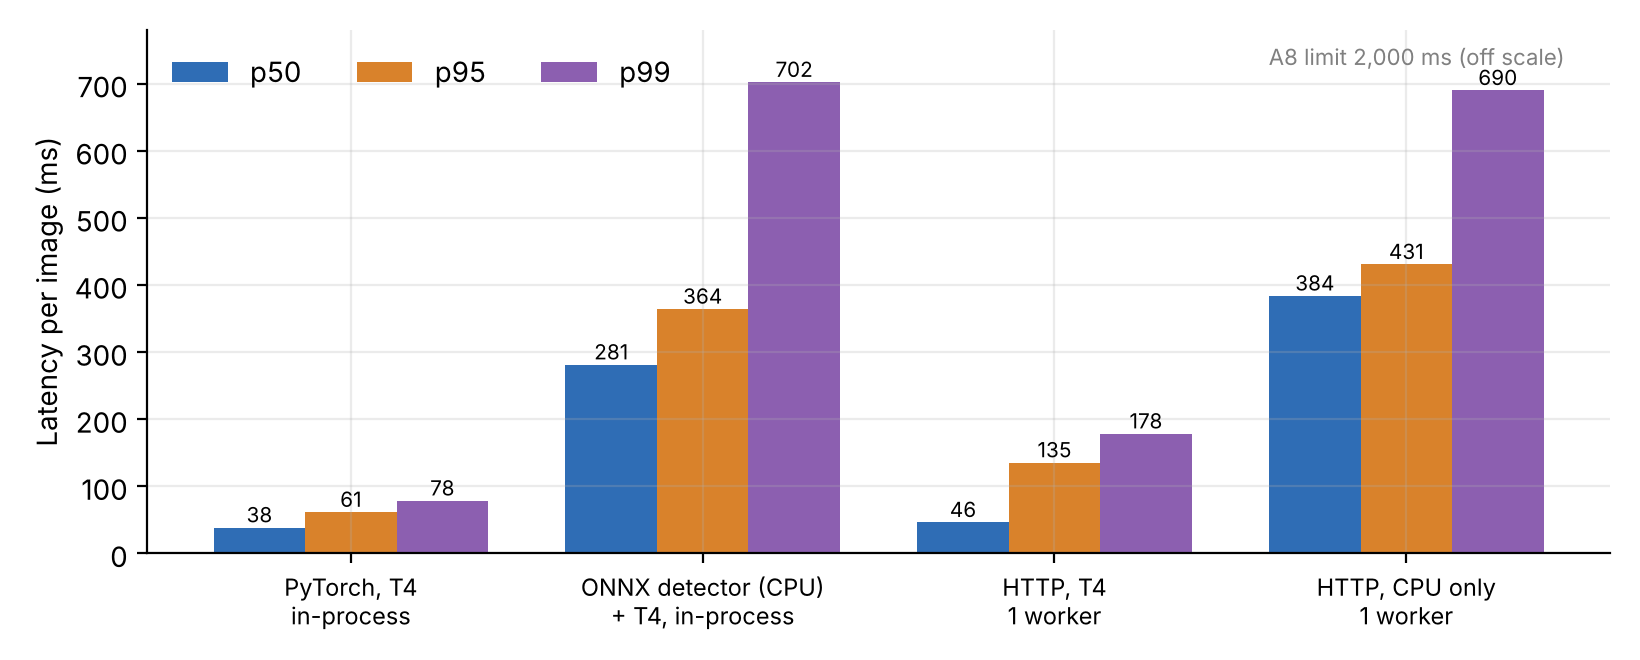
\includegraphics[width=0.8\linewidth]{figures/M8_latency_by_backend.png}
  \caption{Latency percentiles per backend and path (batch 1, FP32; conditions as in the table). CPU and T4 numbers are separate measurements and are not compared; only the in-process T4 PyTorch row is used for A8.}
\end{figure}

\subsection{Verdict against the acceptance criteria}\label{sec:verdict}

\begin{tabularx}{\linewidth}{@{}Y l l l@{}}
\toprule
Criterion & Threshold & Measured & Pass / Fail \\
\midrule
A1 Classification accuracy (test) & $\geq0.90$ & 0.999 & Pass \\
A2 Classification macro-F1 (test) & $\geq0.90$ & 0.999 & Pass \\
A3 Detection mAP50 (test) & $\geq0.75$ & 0.984 & Pass \\
A4 Detection recall at operating point (test) & $\geq0.80$ & 0.959 & Pass \\
A5 Mask mean IoU (test) & $\geq0.75$ & 0.923 & Pass \\
A6 Mask mean Dice (test) & $\geq0.85$ & 0.959 & Pass \\
A7 HTTP success rate (T4) & $\geq0.99$ & 300/300 & Pass \\
A8 p95 latency, T4, batch 1 & $\leq2000$\,ms & 61.4\,ms & Pass \\
A9a ONNX parity, classifier & $\leq0.001$ & $2.98\times10^{-7}$ & Pass \\
A9b ONNX parity, detector & $\leq0.001$ & 0.0018 & \textbf{Fail} \\
\midrule
\multicolumn{3}{@{}l}{\textbf{Preliminary decision}} & \textbf{GO} (PyTorch, staff-supervised) \\
\bottomrule
\end{tabularx}

\smallskip
\textbf{For each FAIL:} A9b: the exported detector's raw head differs by 0.0018--0.0020 and final boxes moved by up to 28.7\,px on 50 real test images; six export and runtime settings did not change this, and the cause is not isolated. The fix at no cost is the one taken: serve the PyTorch detector, which is also about seven times faster here (p50 38.5 vs 281.1\,ms). The decision is therefore GO for a staff-supervised service with PyTorch, and NO-GO for serving the ONNX detector. A diagnostic notebook (\texttt{09\_onnx\_channel\_diagnosis\_v2}) separates box from score channels as a next step.

Main failure modes for the model card: missed small and secondary animals (team photos: recall 0.732; 17 of 52 multi-animal photos marked technically ready because one animal was missed); dark clothed dogs detected as cats; masks spreading into similar-coloured backgrounds. Out of scope: automatic publication, identifying individual animals or people, veterinary use, species other than cats and dogs. Every photo is approved by staff, whatever the verdict.

% =====================================================================
\section{Obstacles and how they were addressed}

\medskip
{\small
\begin{tabularx}{\linewidth}{@{}Y l Y Y l@{}}
\toprule
Obstacle & Module & Impact on the work & Action taken & Status \\
\midrule
Oxford-IIIT Pet has almost only one large, centred animal per photo & M4, M5 & Size and multi-animal behaviour cannot be measured on Oxford & 401 team photos (503 animals) annotated in CVAT and used as an evaluation-only set & Done \\
Detector ONNX export misses the 0.001 parity bound & M8 & ONNX detector cannot be served & PyTorch detector served; six export settings re-checked; diagnosis notebook prepared & Workaround \\
Trimap border pixels are ambiguous & M5 & Mask scores depend on the border convention & Report scores with and without border pixels & Done \\
Weights over 100\,MB and private photos cannot go into Git & M8 & The repository alone cannot run inference & Relative paths in the manifest, SHA-256 checks, weights and photos in private Drive & Done \\
\bottomrule
\end{tabularx}}

\smallskip
\textbf{Support needed before the final presentation (optional):} none.

% =====================================================================
\section{Submission checklist}

\begin{itemize}[leftmargin=1.6em,itemsep=2pt]
  \item[$\checkmark$] Annotations converted and verified visually; data checks reported (\S2.1)
  \item[$\checkmark$] Detector fine-tuned; thresholds swept on validation; operating point justified (\S2.2--2.3)
  \item[$\checkmark$] mAP50, mAP50--95 and per-class AP on the test split; P/R/F1 at the operating point; recall by object size (\S2.4)
  \item[$\checkmark$] False-positive breakdown, FP/FN galleries and at least one detection failure case (\S2.5)
  \item[$\checkmark$] Detector run on images and video at the operating point (\S2.6)
  \item[$\checkmark$] Ground-truth masks checked; segmentation model fine-tuned and compared with a baseline (\S3.1--3.2)
  \item[$\checkmark$] Segmentation evaluated with mask mAP50--95, mIoU and Dice, and one failure case (\S3.4--3.5)
  \item[$\checkmark$] End-to-end pipeline with per-stage timing and a manifest (\S4.1--4.2)
  \item[$\checkmark$] ONNX export with a parity check (\S4.4; detector fails A9b)
  \item[$\checkmark$] Working HTTP service with input and output contracts (\S4.3, \S4.5)
  \item[$\checkmark$] p50/p95/p99 latency, throughput and memory measured with warm-up and stated conditions (\S4.6)
  \item[$\checkmark$] Verdict reported against the acceptance criteria (\S\ref{sec:verdict})
  \item[$\checkmark$] Every figure states split, input resolution and thresholds
  \item[$\checkmark$] No data or personal information committed to the repository (weights, Oxford images and team photos stay in private Drive)
\end{itemize}

% =====================================================================
\section{Self-assessment}

{\small
\begin{tabularx}{\linewidth}{@{}l c c Y Y@{}}
\toprule
Criterion & Max (team of 4) & Self-score & Strongest evidence (section) & Known gap \\
\midrule
Object detection (M4) & 15 & 14 & Test AP per class, sweep on validation, FP taxonomy, team-photo size analysis, video (\S2) & One training recipe only; no comparison with another detector or the COCO model as is \\
Segmentation (M5) & 15 & 13 & Full test mIoU/Dice/mask mAP, matched 300-image SAM baseline, border analysis, failure gallery (\S3) & Mask thresholds not swept on validation; baseline not run on validation \\
Integration and deployment (M8) & 15 & 13 & Manifest, HTTP contracts, T4 and CPU checks, verdict table (\S4) & A9b fails (PyTorch served instead); per-stage percentiles not recorded \\
\midrule
\textbf{Total} & \textbf{45} & \textbf{40} & & \\
\bottomrule
\end{tabularx}}

\end{document}
